\section{Plug-in Models}
\label{section.plugin}

\subsection{Heat Integration}

The Heat Integration Node performs heat integration calculations for the entire process in the meta-flowsheet. This node transfers simulation results to a GAMS-based heat integration program, solves the program, and transfers part of important heat integration results from GAMS to the graphical interface. The detailed heat integration results can be found in \textbackslash gams\textbackslash HeatIntegration.lst. All input and output variables in the nodes connected to the Heat Integration Node (with the edge pointing to the heat integration node) are automatically transferred to heat integration. However, only the variables with heat integration tags are considered and processed in heat integration. Heat integration tags are described in the Heat Integration Tutorial in Section \ref{sec.hi.tut}.

The Heat Integration Node Editor widget is illustrated in Figure \ref{heat.int.inputs} and Figure \ref{heat.int.outputs}. To specify a node as a Heat Integration Node, expand the \bu{Model} section, expand the \bu{Model} drop-down list, and then select ``heat\_integration.'' Some input variables control the performance of heat integration. Output variables display heat integration results, which are used as final results or inputs for steam cycle calculations.

\begin{figure}[H]
	\begin{center}
		\includegraphics[scale=0.55]{Chapt_heat/figs/heat_int_inputs}
		\caption{Heat Integration Node Editor (Input Variables)}
		\label{heat.int.inputs}
	\end{center}
\end{figure}
\clearpage

The Heat Integration Node \bu{Input Variables} are listed below:
\begin{itemize}
	\item Exchanger minimum approach temperature (\bu{EMAT}) is the minimum temperature difference between hot streams and cold streams for heat exchanger area calculations. The value of EMAT is usually not larger than that of HRAT (see below). The default value of EMAT is set to 5K. When a small value of HRAT is chosen (e.g., 3-5K), the value of EMAT should also be small (e.g., 1-3K).
	\item Heat recovery approach temperature (\bu{HRAT}) is the minimum temperature difference between hot streams and cold streams for utility consumption calculations. Smaller HRAT usually leads to lower utility consumptions but higher capital cost of the heat exchanger network. An appropriate value should be selected for HRAT in order to achieve the best economic performance. The typical value of HRAT in industrial applications is 10K, which is also the default value of HRAT. The user may choose other HRAT values depending on their applications (e.g., in power plants, HRAT can be as low as 3-5K for higher heat recovery).
	\item \bu{Life.Plant} is the operating life of the plant. The default value is 20 years. The user can change the value depending on detailed applications.
	\item \bu{Net.Power} is the net power output of a power plant without carbon capture and storage (CCS). This is an optional input variable; therefore, it has no default value. The user only needs to assign a value to it when the steam cycle node is also present in the flowsheet. The net power output is used to calculate the amount of heat recovered for steam cycle via the heat exchanger network.
	\item \bu{No.Stream} is the number of process streams (for heat integration) in the plant. This is an optional input variable without default value. When the value of ``No.Stream'' is not assigned, the number of process streams is calculated by the Python program via heat integration tags (see the Heat Integration Tutorial in Section \ref{sec.hi.tut}).
	\item \bu{Operation.Hours} is the annual operational hours of the plant. For power, refinery, and chemical industries, the typical value is 7500-8500 hours. The default value here is 8000 hours.
	\item \bu{ROR} is the rate of return for the project. The default value is 10 percent. The user should select appropriate values for ROR based on their own projects. The variables \bu{Life.Plant}, \bu{No.Stream}, \bu{Operation.Hours}, and \bu{ROR} are used for the cost calculation. 
\end{itemize}

\begin{figure}[H]
	\begin{center}
		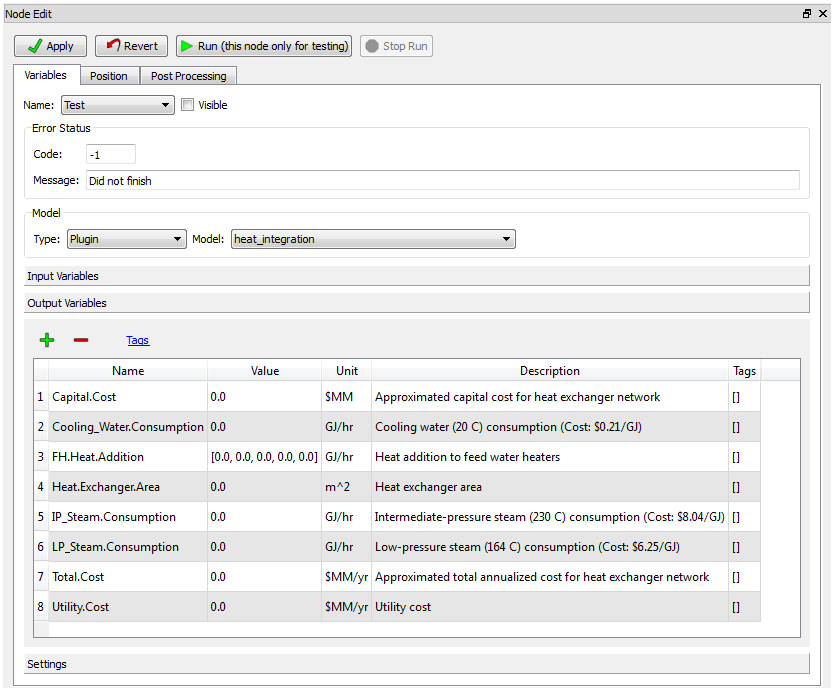
\includegraphics[scale=0.55]{Chapt_heat/figs/heat_int_outputs}
		\caption{Heat Integration Node Editor (Output Variables)}
		\label{heat.int.outputs}
	\end{center}
\end{figure}


The \bu{Output Variables} of the Heat Integration Node are listed below:
\begin{itemize}
	\item \bu{Capital.Cost} is the minimum approximated capital cost for the heat exchanger network (in million U.S. dollars). The capital cost is calculated from the heat exchanger area (see below).
	\item \bu{Cooling.Water.Consumption} is the minimum cooling water consumption rate (represented by energy rate GJ/hr) predicted by heat integration. Cooling water is an outside utility with the temperature of 20\degree C.
	\item \bu{FH.Heat.Addition} is the amount of heat recovered to feed water heaters in the steam cycle. This variable is only valid when steam cycle calculations are also presented. If more heat is added to the steam cycle, higher net power output is expected. The value of ``FH.Heat.Addition'' is a vector with five elements. The first to fifth element of the vector represents the amount of heat added to the first-stage to the fifth-stage of the feed water heater in the steam cycle. The temperature of the feed water increases from the first-stage to the fifth-stage; therefore, heat added to the feed water heaters achieves a higher efficiency power generation from the first-stage to the fifth-stage heater. The temperature range for the five feed water heaters are 34-65\degree C, 65-96\degree C, 96-128\degree C, 128-160\degree C, and 160-195\degree C. These values are obtained from a supercritical power plant simulation model in Thermoflex.
	\item \bu{Heat.Exchanger.Area} is the minimum heat exchanger area (in square meters), which is used for the capital cost calculation.
	\item \bu{IP\_Steam.Consumption} is the minimum intermediate-pressure steam consumption rate (in GJ/hr). Note: Both intermediate- and low-pressure steam are treated as a utility in heat integration calculations here; however, they are actually extracted from the steam cycle in the power plant. Therefore, minimizing steam consumption is equivalent to maximizing the net power output. Intermediate-pressure steam is extracted from the crossover of the pressurized intermediate-pressure turbine (PIPT) and the intermediate-pressure turbine (IPT) with the temperature of 230\degree C.
	\item \bu{LP\_Steam.Consumption} is the minimum low-pressure steam consumption rate (in GJ/hr). Low-pressure steam is extracted from the crossover of IPT and low-pressure steam turbine (LPT) with the temperature of 164\degree C.
	\item \bu{Total.Cost} is the minimum approximated total annualized cost for the heat exchanger network (in million U.S. dollars per year), which equals the sum of utility cost and annualized capital cost.
	\item \bu{Utility.Cost} is the minimum utility cost (in million U.S. dollars per year), which equals the sum of the cost of cooling water, intermediate-pressure steam, and low-pressure steam. It can also be treated as scaled total utility consumption where the consumption rate of each utility is weighted by its cost.
\end{itemize}

\subsection{Steam Cycle}

The Steam Cycle Node performs steam cycle and power output calculations for a power plant with CCS (and possibly heat integration). Correlations for net power output with steam extraction and heat addition to feed water heaters, which are obtained from a supercritical power plant model in Thermoflex, are utilized to calculate net power output and net efficiency with CCS in the Steam Cycle Node. These correlations are currently hard coded in Python for this node. The users will have a choice to provide their own correlations in future versions of FOQUS. 

The Steam Cycle Node Editor widget is illustrated in Figure \ref{steam.cycle.inputs} and Figure \ref{steam.cycle.outputs}. 

To specify a node as a Steam Cycle Node, expand the \bu{Model} section, click on the \bu{Model} drop-down list, and then select ``steam\_cycle.'' All input variables (potentially) can be contributed to power output calculations; however, not all input variables are required to have a value assigned, except net power output and net efficiency without CCS. Output variables describe effects of CCS and heat integration to net power output and net efficiency.

\begin{figure}[H]
	\begin{center}
		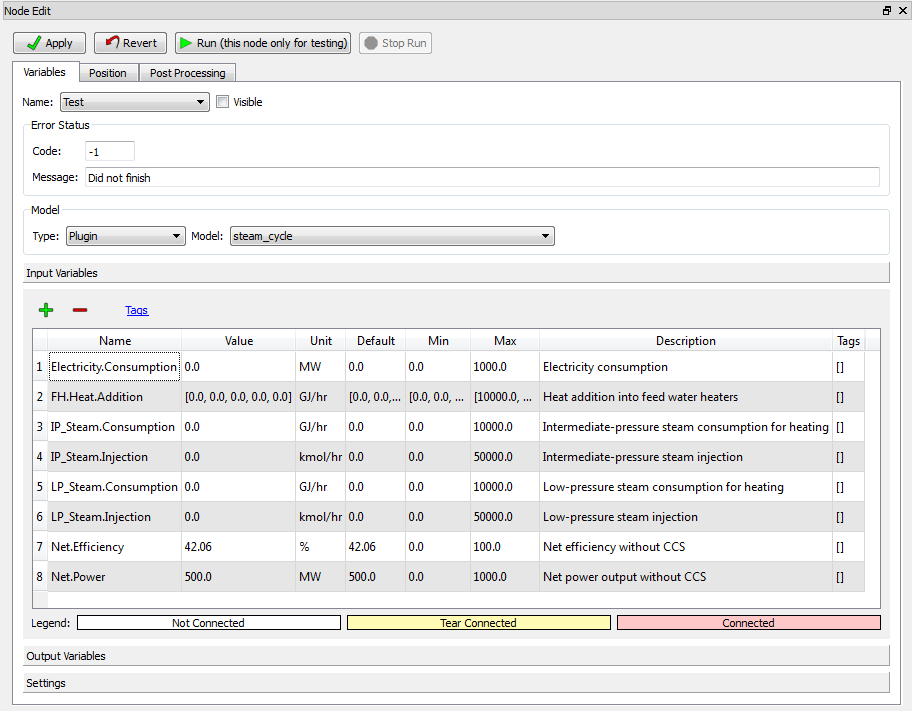
\includegraphics[scale=0.55]{Chapt_heat/figs/steam_cycle_inputs}
		\caption{Steam Cycle Node Editor (Input Variables)}
		\label{steam.cycle.inputs}
	\end{center}
\end{figure}

The \bu{Input Variables} of the Steam Cycle Node are described below:
\begin{itemize}
	\item \bu{Electricity.Consumption} is the total electricity consumption in all processes other than steam cycle. The input value of this variable can be provided by the user or transferred from simulation outputs.
	\item \bu{FH.Heat.Addition} is the amount of heat recovered to feed water heaters in steam cycle. The input value of this variable can be transferred from heat integration output.
	\item \bu{IP\_Steam.Consumption} is the intermediate-pressure steam consumption rate in heat exchangers. It is usually provided by heat integration, and sometimes it can be directly provided by simulation.
	\item \bu{IP\_Steam.Injection} is the intermediate-pressure steam injection rate to process streams. In some equipment, such as regenerators in the capture process, steam needs to be injected directly into the input stream to provide a large amount of heat and realize fast heat transfer. The steam injection rate is different from the steam consumption rate as it does not need heat exchangers and is not considered in heat integration. This variable is typically provided by simulation output.
	\item \bu{LP\_Steam.Consumption} is the low-pressure steam consumption rate in heat exchangers provided by heat integration or simulation output.
	\item \bu{LP\_Steam.Injection} is the low-pressure steam injection rate to process \\streams provided by simulation output.
	\item \bu{Net.Efficiency} is the net efficiency of the power plant without CCS. Its default value is 42.06 percent, which is the efficiency of a typical supercritical pulverized coal-fired power plant without CCS. The user should change the value when another type of power plant is applied.
	\item \bu{Net.Power} is the net power output of a power plant without CCS. The user must give an input to this variable to perform steam cycle calculations. Both \bu{Net.Efficiency} and \bu{Net.Power} provide base case values for a power plant without CCS and heat integration.
\end{itemize}

\begin{figure}[H]
	\begin{center}
		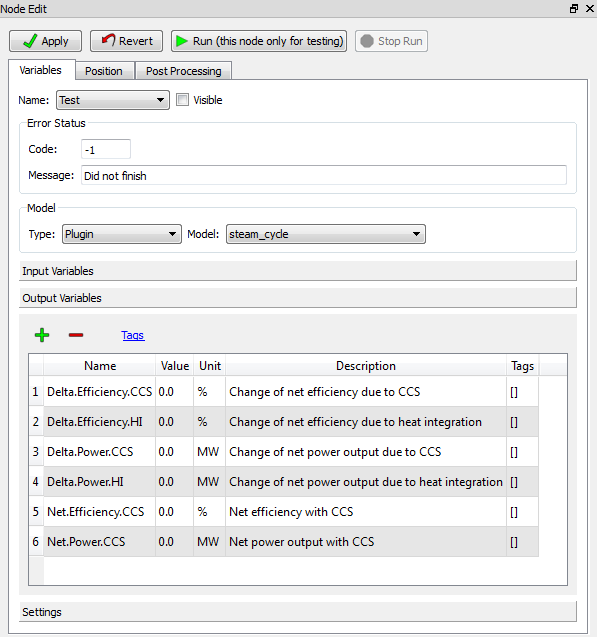
\includegraphics[scale=0.55]{Chapt_heat/figs/steam_cycle_outputs}
		\caption{Steam Cycle Node Editor (Output Variables)}
		\label{steam.cycle.outputs}
	\end{center}
\end{figure}

The \bu{Output Variables} of the Steam Cycle Node are listed below:
\begin{itemize}
	\item \bu{Delta.Efficiency.CCS} is the change of the net efficiency of a power plant with CCS compared to the base case value. This variable is expected to be negative since CCS decreases the net power output to a certain degree.
	\item \bu{Delta.Efficiency.HI} is the change of the net efficiency of a power plant with heat integration compared to the base case value. This variable is expected to be positive since heat integration potentially increases the net power output.
	\item \bu{Delta.Power.CCS} is the change of the net power output of a power plant with CCS compared to the base case value.
	\item \bu{Delta.Power.HI} is the change of the net power output of a power plant with CCS compared to the base case value.
	\item \bu{Net.Efficiency.CCS} is the net efficiency of the power plant with CCS given the base case value.
	\item \bu{Net.Power.CCS} is the net power output of the power plant with CCS assigned as the base case value.
\end{itemize}

